\documentclass[10pt,twoside]{article}
\usepackage[T1]{fontenc}
\usepackage[utf8]{inputenc}
\usepackage{helvet}
\renewcommand{\familydefault}{\sfdefault}
\usepackage{geometry}
\geometry{paperwidth=6.93in,paperheight=9.11in,inner=0.56in,outer=0.46in,top=0.66in,bottom=0.66in,headheight=14pt}
\usepackage{amsmath}
\usepackage{array}
\usepackage{booktabs}
\usepackage{longtable}
\usepackage{tabularx}
\usepackage{xcolor}
\usepackage{tikz}
\usetikzlibrary{decorations.pathreplacing,decorations.pathmorphing}
\usepackage{fancyhdr}
\usepackage{titlesec}
\usepackage{enumitem}
\usepackage{needspace}
\usepackage{hyperref}
\hypersetup{colorlinks=true,linkcolor=black,urlcolor=black,pdfauthor={ISA tooling},pdftitle={Bedrock Programmer's Reference Manual}}
\makeatletter
\renewcommand{\@pnumwidth}{2.2em}
\renewcommand{\@tocrmarg}{3.0em}
\makeatother
\definecolor{RuleGray}{gray}{0.18}
\definecolor{LightRule}{gray}{0.80}
\setlength{\parindent}{0pt}
\setlength{\parskip}{4pt}
\setlength{\tabcolsep}{2pt}
\sloppy
\emergencystretch=2em
\clubpenalty=10000
\widowpenalty=10000
\displaywidowpenalty=10000
\brokenpenalty=10000
\raggedbottom
\setlist[itemize]{leftmargin=1.0em,itemsep=1pt,topsep=2pt}
\renewcommand{\arraystretch}{1.12}
\pagestyle{fancy}
\fancyhf{}
\fancyhead[LE]{\small Bedrock}
\fancyhead[RO]{\small PROGRAMMER'S REFERENCE MANUAL}
\fancyfoot[LE,RO]{\small\thepage}
\fancyfoot[LO,RE]{\small Bedrock ARCHITECTURE}
\renewcommand{\headrulewidth}{0.35pt}
\renewcommand{\footrulewidth}{0pt}
\titleformat{\section}{\large\bfseries\MakeUppercase}{\thesection}{0.7em}{}
\titleformat{\subsection}{\normalsize\bfseries}{\thesubsection}{0.6em}{}
\titlespacing*{\section}{0pt}{1.2em}{0.7em}
\titlespacing*{\subsection}{0pt}{1.0em}{0.45em}
\newcounter{manualfigure}[section]
\newcounter{manualtable}[section]
\renewcommand{\themanualfigure}{\thesection-\arabic{manualfigure}}
\renewcommand{\themanualtable}{\thesection-\arabic{manualtable}}
\newcommand{\manualfield}[2]{%
  \par\noindent\begin{tabularx}{\linewidth}{@{}>{\raggedright\arraybackslash}p{1.46in}X@{}}%
  \textbf{#1} & #2%
  \end{tabularx}\par\vspace{2pt}}
\newcommand{\manualblockfield}[2]{%
  \par\Needspace{0.45in}%
  \begin{description}[style=multiline,leftmargin=1.46in,labelwidth=1.32in,labelsep=0.14in,%
    topsep=0pt,partopsep=0pt,itemsep=0pt,parsep=0pt]%
  \item[\textbf{#1}] #2%
  \end{description}\vspace{2pt}}
\newenvironment{manualraggedblock}{%
  \begingroup\raggedright
}{%
  \par\endgroup}
\newenvironment{manuallongtable}[1]{%
  \begingroup\footnotesize
  \setlength{\LTpre}{2pt}%
  \setlength{\LTpost}{2pt}%
  \begin{longtable}{#1}%
}{%
  \end{longtable}%
  \endgroup}
\newenvironment{manualdenselongtable}[1]{%
  \begingroup\scriptsize
  \setlength{\tabcolsep}{2pt}%
  \setlength{\LTpre}{2pt}%
  \setlength{\LTpost}{2pt}%
  \begin{longtable}{#1}%
}{%
  \end{longtable}%
  \endgroup}
\newenvironment{manualtabular}[1]{%
  \Needspace{1.25in}%
  \begingroup\footnotesize
  \begin{center}%
  \begin{tabular}{#1}%
}{%
  \end{tabular}%
  \end{center}%
  \endgroup}
\newenvironment{manualformblock}[1]{%
  \Needspace{#1}%
  \par\vspace{7pt}\begingroup\footnotesize
}{%
  \par\endgroup}
\newenvironment{manualtikzdiagram}[4]{%
  \begingroup
  \Needspace{#1}%
  \def\manualtikzdiagramcaption{#4}%
  \begin{center}\vspace{3pt}%
  \begin{tikzpicture}[x=#2,y=#3,every node/.style={font=\scriptsize}]%
}{%
  \end{tikzpicture}%
  \manualcaption{\manualtikzdiagramcaption}%
  \end{center}%
  \endgroup}
\newenvironment{manuallistedtikzdiagram}[4]{%
  \begingroup
  \Needspace{#1}%
  \def\manualtikzdiagramcaption{#4}%
  \begin{center}\vspace{3pt}%
  \begin{tikzpicture}[x=#2,y=#3,every node/.style={font=\scriptsize}]%
}{%
  \end{tikzpicture}%
  \manualfigurecaption{\manualtikzdiagramcaption}%
  \end{center}%
  \endgroup}
\newif\ifmanualbitdiagrammeasuring
\newif\ifmanualbitrowmeasuring
\newcount\manualbitdiagramrows
\newcount\manualbitdiagrammaxbits
\newcount\manualbitrowbits
\newcount\manualbitrowindex
\newcount\manualbitfieldx
\newcount\manualbitfieldwidth
\newcommand{\manualbitfield}[2]{%
  \manualbitfieldwidth=#2\relax
  \ifmanualbitrowmeasuring
    \advance\manualbitrowbits by \manualbitfieldwidth
  \else
    \draw ({\the\manualbitfieldx},{\manualbitrowy}) rectangle
      ({\the\numexpr\manualbitfieldx+\manualbitfieldwidth\relax},{\manualbitrowy + 1});
    \node at ({\the\manualbitfieldx + #2/2},{\manualbitrowy + 0.5}) {#1};
    \advance\manualbitfieldx by \manualbitfieldwidth
  \fi}
\newcommand{\manualbitfieldcode}[2]{\manualbitfield{\texttt{#1}}{#2}}
\newcommand{\manualbitfieldtext}[2]{\manualbitfield{#1}{#2}}
\newcommand{\manualbitlabel}[1]{%
  \ifmanualbitrowmeasuring
  \else
    \pgfmathsetmacro{\manualbitlabelx}{\the\manualbitrowbits-(#1)-0.5}%
    \node[anchor=south] at ({\manualbitlabelx},{\manualbitrowy + 1.18}) {#1};%
  \fi}
\newcommand{\manualbitdefaultlabels}{%
  \node[anchor=south] at (0,{\manualbitrowy + 1.18}) {\the\numexpr\manualbitrowbits-1\relax};%
  \node[anchor=south] at (\the\manualbitrowbits,{\manualbitrowy + 1.18}) {0};%
}
\newcommand{\manualbitrowbody}[4]{%
  \manualbitrowbits=0
  \manualbitrowmeasuringtrue#3\manualbitrowmeasuringfalse
  \ifmanualbitdiagrammeasuring
    \advance\manualbitdiagramrows by 1
    \ifnum\manualbitrowbits>\manualbitdiagrammaxbits
      \manualbitdiagrammaxbits=\manualbitrowbits
    \fi
  \else
    \pgfmathsetmacro{\manualbitrowy}{-2.08*\the\manualbitrowindex}
    \node[anchor=east] at (-0.35,{\manualbitrowy + 0.5}) {#1};
    #2
    \ifnum#4>0
      \ifnum\manualbitrowbits>15
        \foreach \manualbittick in {4,8,...,\the\numexpr\manualbitrowbits-1\relax} {%
          \draw[LightRule] (\manualbittick,\manualbitrowy) -- (\manualbittick,{\manualbitrowy + 1});}
      \fi
    \fi
    \manualbitfieldx=0
    #3
    \advance\manualbitrowindex by 1
  \fi}
\newcommand{\manualbitrowwithlabels}[3]{\manualbitrowbody{#1}{#2}{#3}{1}}
\newcommand{\manualbitfieldrow}[3]{\manualbitrowbody{#1}{#2}{#3}{0}}
\newcommand{\manualbitrow}[2]{\manualbitrowwithlabels{#1}{\manualbitdefaultlabels}{#2}}
\newcommand{\manualrenderbitdiagram}[3]{%
  \begingroup
  \manualbitdiagramrows=0
  \manualbitdiagrammaxbits=0
  \manualbitdiagrammeasuringtrue#2\manualbitdiagrammeasuringfalse
  \pgfmathsetmacro{\manualbitdiagramneedspace}{0.80 + 0.45*\the\manualbitdiagramrows}
  \pgfmathsetmacro{\manualbitdiagramxscale}{min(0.30, 4.70/\the\manualbitdiagrammaxbits)}
  \Needspace{\manualbitdiagramneedspace in}%
  \begin{center}\vspace{3pt}%
  \begin{tikzpicture}[x=\manualbitdiagramxscale in,y=0.22in,every node/.style={font=\scriptsize}]%
  \manualbitrowindex=0
  #2
  \end{tikzpicture}%
  #3{#1}%
  \end{center}%
  \endgroup}
\NewDocumentEnvironment{manualbitdiagram}{m +b}{%
  \manualrenderbitdiagram{#1}{#2}{\manualcaption}%
}{}
\NewDocumentEnvironment{manuallistedbitdiagram}{m +b}{%
  \manualrenderbitdiagram{#1}{#2}{\manualfigurecaption}%
}{}
\newif\ifmanualformatdiagrammeasuring
\newif\ifmanualformatrowmeasuring
\newcount\manualformatdiagramrows
\newcount\manualformatdiagrammaxunits
\newcount\manualformatrowbits
\newcount\manualformatrowunits
\newcount\manualformatrowindex
\newcount\manualformatfieldbits
\newcount\manualformatfieldunits
\newcount\manualformatfieldx
\newcount\manualformatfieldhigh
\newcount\manualformatrowlow
\newcount\manualformatfieldminunits
\newcommand{\manualformatfield}[2]{%
  \manualformatfieldbits=#2\relax
  \manualformatfieldunits=\manualformatfieldbits
  \ifnum\manualformatfieldunits<\manualformatfieldminunits
    \manualformatfieldunits=\manualformatfieldminunits
  \fi
  \ifmanualformatrowmeasuring
    \advance\manualformatrowbits by \manualformatfieldbits
    \advance\manualformatrowunits by \manualformatfieldunits
  \else
    \ifnum\manualformatfieldhigh>\manualformatrowlow
      \ifnum\manualformatfieldbits=1
        \node[anchor=south east] at ({\the\numexpr\manualformatfieldx+\manualformatfieldunits\relax},{\manualformatrowy + 1.18}) {\the\manualformatfieldhigh};
      \else
        \node[anchor=south] at ({\the\manualformatfieldx},{\manualformatrowy + 1.18}) {\the\manualformatfieldhigh};
      \fi
    \fi
    \draw ({\the\manualformatfieldx},{\manualformatrowy}) rectangle
      ({\the\numexpr\manualformatfieldx+\manualformatfieldunits\relax},{\manualformatrowy + 1});
    \node at ({\the\manualformatfieldx + \the\manualformatfieldunits/2},{\manualformatrowy + 0.5}) {#1};
    \advance\manualformatfieldx by \manualformatfieldunits
    \advance\manualformatfieldhigh by -\manualformatfieldbits
  \fi}
\newcommand{\manualformatfieldcode}[2]{\manualformatfield{\texttt{#1}}{#2}}
\newcommand{\manualformatrowrange}[4]{%
  \manualformatrowbits=0
  \manualformatrowunits=0
  \manualformatrowmeasuringtrue#4\manualformatrowmeasuringfalse
  \ifmanualformatdiagrammeasuring
    \advance\manualformatdiagramrows by 1
    \ifnum\manualformatrowunits>\manualformatdiagrammaxunits
      \manualformatdiagrammaxunits=\manualformatrowunits
    \fi
  \else
    \pgfmathsetmacro{\manualformatrowy}{-2.08*\the\manualformatrowindex}
    \node[anchor=east] at (-0.35,{\manualformatrowy + 0.5}) {#1};
    \manualformatfieldx=0
    \manualformatrowlow=#3\relax
    \manualformatfieldhigh=#2\relax
    #4
    \node[anchor=south east] at ({\the\manualformatfieldx},{\manualformatrowy + 1.18}) {#3};
    \advance\manualformatrowindex by 1
  \fi}
\newcommand{\manualformatrow}[2]{%
  \manualformatrowbits=0
  \manualformatrowunits=0
  \manualformatrowmeasuringtrue#2\manualformatrowmeasuringfalse
  \manualformatrowrange{#1}{\number\numexpr\manualformatrowbits-1\relax}{0}{#2}}
\newcommand{\manualrenderformatdiagram}[4]{%
  \begingroup
  \manualformatfieldminunits=#2\relax
  \manualformatdiagramrows=0
  \manualformatdiagrammaxunits=0
  \manualformatdiagrammeasuringtrue#3\manualformatdiagrammeasuringfalse
  \pgfmathsetmacro{\manualformatdiagramneedspace}{0.80 + 0.45*\the\manualformatdiagramrows}
  \pgfmathsetmacro{\manualformatdiagramxscale}{min(0.30, 4.70/\the\manualformatdiagrammaxunits)}
  \Needspace{\manualformatdiagramneedspace in}%
  \begin{center}\vspace{3pt}%
  \begin{tikzpicture}[x=\manualformatdiagramxscale in,y=0.22in,every node/.style={font=\scriptsize}]%
  \manualformatrowindex=0
  #3
  \end{tikzpicture}%
  #4{#1}%
  \end{center}%
  \endgroup}
\NewDocumentEnvironment{manualformatdiagram}{m m +b}{%
  \manualrenderformatdiagram{#1}{#2}{#3}{\manualcaption}%
}{}
\NewDocumentEnvironment{manuallistedformatdiagram}{m m +b}{%
  \manualrenderformatdiagram{#1}{#2}{#3}{\manualfigurecaption}%
}{}
\newif\ifmanualbyteordermeasuring
\newcount\manualbyteordercells
\newcount\manualbyteordercellindex
\newcommand{\manualbytecell}[2]{%
  \ifmanualbyteordermeasuring
    \advance\manualbyteordercells by 1
  \else
    \draw ({\the\manualbyteordercellindex},0) rectangle
      ({\the\numexpr\manualbyteordercellindex+1\relax},1);
    \node at ({\the\manualbyteordercellindex + 0.5},0.62) {#1};
    \node[anchor=north] at ({\the\manualbyteordercellindex + 0.5},-0.04) {\texttt{#2}};
    \advance\manualbyteordercellindex by 1
  \fi}
\newcommand{\manualrenderbyteorderdiagram}[8]{%
  \begingroup
  \manualbyteordercells=0
  \manualbyteordermeasuringtrue#7\manualbyteordermeasuringfalse
  \pgfmathsetmacro{\manualbyteorderxscale}{min(0.72, 4.70/\the\manualbyteordercells)}
  \Needspace{1.35in}%
  \begin{center}\vspace{3pt}%
  \begin{tikzpicture}[x=\manualbyteorderxscale in,y=0.34in,every node/.style={font=\scriptsize}]%
  \manualbyteordercellindex=0
  #7
  \node[anchor=east] at (-0.15,0.62) {#2};
  \node[anchor=east] at (-0.15,-0.20) {#3};
  \draw[->] (0,-0.70) -- node[below] {#4} (\the\manualbyteordercells,-0.70);
  \node[anchor=west] at (0,1.22) {#5};
  \node[anchor=east] at (\the\manualbyteordercells,1.22) {#6};
  \end{tikzpicture}%
  #8{#1}%
  \end{center}%
  \endgroup}
\NewDocumentEnvironment{manualbyteorderdiagram}{m m m m m m +b}{%
  \manualrenderbyteorderdiagram{#1}{#2}{#3}{#4}{#5}{#6}{#7}{\manualcaption}%
}{}
\NewDocumentEnvironment{manuallistedbyteorderdiagram}{m m m m m m +b}{%
  \manualrenderbyteorderdiagram{#1}{#2}{#3}{#4}{#5}{#6}{#7}{\manualfigurecaption}%
}{}
\newif\ifmanualstackframemeasuring
\newcount\manualstackframerows
\newcount\manualstackframerowindex
\newcommand{\manualstackframewidth}{3.25}
\newcommand{\manualstackframerowheight}{0.50}
\newcommand{\manualstackframeslotbody}[4]{%
  \ifmanualstackframemeasuring
    \advance\manualstackframerows by 1
  \else
    \pgfmathsetmacro{\manualstackframey}{-\manualstackframerowheight*\the\manualstackframerowindex}%
    \pgfmathsetmacro{\manualstackframemidy}{\manualstackframey - \manualstackframerowheight/2}%
    \ifnum#4>0
      \node[anchor=east] at (-0.44,\manualstackframemidy) {SP};%
      \draw[->] (-0.40,\manualstackframemidy) -- (-0.02,\manualstackframemidy);%
    \else
      \node[anchor=east] at (-0.08,\manualstackframemidy) {\texttt{#1}};%
    \fi
    \ifnum#3>0
      \draw[densely dashed] (0,{\manualstackframey - \manualstackframerowheight}) -- (0,\manualstackframey) -- (\manualstackframewidth,\manualstackframey) -- (\manualstackframewidth,{\manualstackframey - \manualstackframerowheight});%
    \else
      \draw (0,\manualstackframey) rectangle (\manualstackframewidth,{\manualstackframey - \manualstackframerowheight});%
    \fi
    \node at ({\manualstackframewidth/2},\manualstackframemidy) {#2};%
    \advance\manualstackframerowindex by 1
  \fi}
\newcommand{\manualstackframeslot}[2]{\manualstackframeslotbody{#1}{#2}{0}{0}}
\newcommand{\manualstackframespslot}[2]{\manualstackframeslotbody{#1}{#2}{0}{1}}
\newcommand{\manualstackframepayload}[2]{\manualstackframeslotbody{#1}{#2}{1}{0}}
\newcommand{\manualrenderstackframediagram}[3]{%
  \begingroup
  \manualstackframerows=0
  \manualstackframemeasuringtrue#2\manualstackframemeasuringfalse
  \pgfmathsetmacro{\manualstackframeneedspace}{0.95 + 0.18*\the\manualstackframerows}%
  \Needspace{\manualstackframeneedspace in}%
  \begin{center}\vspace{3pt}%
  \begin{tikzpicture}[x=1in,y=0.30in,every node/.style={font=\scriptsize}]%
  \node[anchor=south] at (0.00,0.26) {63};%
  \node[anchor=south] at (\manualstackframewidth,0.26) {0};%
  \manualstackframerowindex=0
  #2
  \end{tikzpicture}%
  #3{#1}%
  \end{center}%
  \endgroup}
\NewDocumentEnvironment{manualstackframediagram}{m +b}{%
  \manualrenderstackframediagram{#1}{#2}{\manualcaption}%
}{}
\NewDocumentEnvironment{manuallistedstackframediagram}{m +b}{%
  \manualrenderstackframediagram{#1}{#2}{\manualfigurecaption}%
}{}
\newcommand{\manualifempty}[3]{%
  \if\relax\detokenize{#1}\relax
    #2%
  \else
    #3%
  \fi}
\newcommand{\manualeaflowstart}[2]{%
  \begingroup
  \Needspace{#1}%
  \def\manualeaflowcaption{#2}%
  \begin{center}\vspace{2pt}%
  \begin{tikzpicture}[x=1in,y=1in,every node/.style={font=\scriptsize},>=stealth]%
}
\newcommand{\manualeaflowend}{%
  \end{tikzpicture}%
  \manualcaption{\manualeaflowcaption}%
  \end{center}%
  \endgroup}
\newcommand{\manualeaflowrowlabel}[4]{%
  \node[anchor=west] at (0.02,#2) {#1};
  \draw (#3,#2) -- (#4,#2);}
\newcommand{\manualeaflowbox}[6]{%
  \node[draw,align=center,minimum width=#4in,minimum height=0.26in] (#1) at (#2,#3) {#5};
  \ifnum#6>0
    \node[anchor=south] at ({#2 - #4/2},{#3 + 0.16}) {63};
    \node[anchor=south] at ({#2 + #4/2},{#3 + 0.16}) {0};
  \fi}
\newcommand{\manualeaflowlabeledbox}[7]{%
  \pgfmathsetmacro{\manualeaflowleft}{#4 - #5/2}%
  \manualeaflowrowlabel{#1}{#3}{1.55}{\manualeaflowleft}%
  \manualeaflowbox{#2}{#4}{#3}{#5}{#6}{#7}}
\newcommand{\manualeaflowcircle}[4]{%
  \node[draw,circle,inner sep=0pt,minimum size=0.27in] (#1) at (#2,#3) {#4};}
\newcommand{\manualeaflowmemorytail}[4]{%
  \manualeaflowlabeledbox{MEMORY}{mem}{#2}{#3}{#4}{OPERAND}{0}%
  \draw[->] (#1.south) -- node[midway,right] {POINTS TO} (mem.north);}
\newcommand{\manualeadirectflow}[4]{%
  \manualeaflowstart{1.55in}{#1}%
  \manualeaflowlabeledbox{#2}{reg}{0.18}{3.82}{3.05}{#3}{1}%
  \manualeaflowlabeledbox{OPERAND}{operand}{-0.62}{3.82}{3.05}{#4}{0}%
  \draw[->] (reg.south) -- (operand.north);%
  \manualeaflowend}
\newcommand{\manualeaimmediateflow}[3]{%
  \manualeaflowstart{1.55in}{#1}%
  \manualeaflowlabeledbox{IMMEDIATE DATA}{imm}{0.20}{3.82}{3.05}{#2}{1}%
  \manualeaflowlabeledbox{OPERAND}{operand}{-0.62}{3.82}{3.05}{#3}{0}%
  \draw[->] (imm.south) -- (operand.north);%
  \manualeaflowend}
\newcommand{\manualeasimplememoryflow}[4]{%
  \manualeaflowstart{2.10in}{#1}%
  \manualeaflowlabeledbox{#2}{src}{0.18}{3.82}{3.05}{#3}{1}%
  \manualeaflowlabeledbox{OPERAND POINTER}{ptr}{-0.64}{3.82}{3.05}{#4}{1}%
  \draw[->] (src.south) -- (ptr.north);%
  \manualeaflowmemorytail{ptr}{-1.42}{3.82}{3.10}%
  \manualeaflowend}
\newcommand{\manualeaadditivememoryflow}[5]{%
  \manualeaflowstart{2.35in}{#1}%
  \manualeaflowlabeledbox{#2}{base}{0.72}{4.62}{2.25}{#3}{1}%
  \manualeaflowlabeledbox{DISPLACEMENT}{disp}{-0.10}{3.20}{2.05}{#4}{1}%
  \manualeaflowcircle{add}{4.62}{-0.10}{+}%
  \manualeaflowlabeledbox{OPERAND POINTER}{ptr}{-0.94}{4.62}{2.25}{#5}{1}%
  \draw[->] (base.south) -- (add.north);%
  \draw[->] (disp.east) -- (add.west);%
  \draw[->] (add.south) -- (ptr.north);%
  \manualeaflowmemorytail{ptr}{-1.72}{4.62}{2.25}%
  \manualeaflowend}
\newcommand{\manualeaindexedmemoryflow}[6]{%
  \manualeaflowstart{3.30in}{#1}%
  \manualeaflowlabeledbox{#2}{base}{0.92}{4.48}{2.38}{#3}{1}%
  \manualeaflowcircle{addindex}{4.48}{-1.18}{+}%
  \manualifempty{#4}{%
    \draw[->] (base.south) -- (addindex.north);%
  }{%
    \manualeaflowlabeledbox{DISPLACEMENT}{disp}{0.22}{3.22}{2.15}{#4}{1}%
    \manualeaflowcircle{addbase}{4.48}{0.22}{+}%
    \draw[->] (base.south) -- (addbase.north);%
    \draw[->] (disp.east) -- (addbase.west);%
    \draw[->] (addbase.south) -- (addindex.north);%
  }%
  \manualeaflowlabeledbox{INDEX REGISTER}{idx}{-0.48}{3.42}{1.85}{#5}{1}%
  \manualeaflowlabeledbox{SCALE}{scale}{-1.18}{2.48}{1.35}{SCALE VALUE}{0}%
  \manualeaflowcircle{mul}{3.42}{-1.18}{x}%
  \manualeaflowlabeledbox{OPERAND POINTER}{ptr}{-1.62}{4.48}{2.38}{#6}{1}%
  \draw[->] (idx.south) -- (mul.north);%
  \draw[->] (scale.east) -- (mul.west);%
  \draw[->] (mul.east) -- (addindex.west);%
  \draw[->] (addindex.south) -- (ptr.north);%
  \manualeaflowmemorytail{ptr}{-2.40}{4.48}{2.38}%
  \manualeaflowend}
\newcommand{\manualcaption}[1]{\par\smallskip\centerline{\small\bfseries #1}\smallskip}
\newcommand{\manualfigurecaption}[1]{%
  \refstepcounter{manualfigure}\phantomsection\addcontentsline{lof}{figure}{\protect\numberline{\themanualfigure}#1}%
  \par\smallskip\centerline{\small\bfseries Figure \themanualfigure. #1}\smallskip}
\newcommand{\manualtablecaption}[1]{%
  \refstepcounter{manualtable}\phantomsection\addcontentsline{lot}{table}{\protect\numberline{\themanualtable}#1}%
  \par\smallskip\centerline{\small\bfseries Table \themanualtable. #1}\smallskip}
\newcommand{\instrhead}[3]{%
  \phantomsection#3%
  \Needspace{1.3in}
  \noindent\begin{tabular*}{\linewidth}{@{}l@{\extracolsep{\fill}}c r@{}}%
  {\Large\bfseries #1} & {\bfseries #2} & {\Large\bfseries #1}\\%
  \end{tabular*}
  \vspace{4pt}\hrule height 0.45pt\vspace{9pt}}
\newenvironment{manualinstruction}[3]{%
  \instrhead{#1}{#2}{\label{#3}}%
}{%
  \par}
\newcommand{\manualinstructionfield}[2]{\manualblockfield{#1:}{#2}}
\newcommand{\manualinstructionstatus}[2]{\manualblockfield{#1:}{#2}}
\newenvironment{manualinstructionformat}{%
  \par\noindent\textbf{Instruction Format:}\par
}{%
  \par}
\newenvironment{manualinstructionforms}{%
  \par\vspace{6pt}\noindent\textbf{Instruction Forms:}\par
}{%
  \par}
\newenvironment{manualcode}{\par\small\ttfamily\begin{tabularx}{\linewidth}{@{}X@{}}}{\end{tabularx}\par}
\newcolumntype{Y}{>{\raggedright\arraybackslash}X}
\newcolumntype{Z}{>{\raggedright\arraybackslash\ttfamily\footnotesize}X}
\begin{document}

\thispagestyle{empty}
\begin{center}
{\Large\bfseries Bedrock Programmer's Reference Manual}\\[4pt]
{\large SAVE/RESTORE Processor-State Save Area Preview}
\end{center}
\vspace{0.25in}
\setcounter{section}{5}
\clearpage
\section{SAVE/RESTORE Processor-State Save Area}
\par\smallskip
\Needspace{5.88in}
\noindent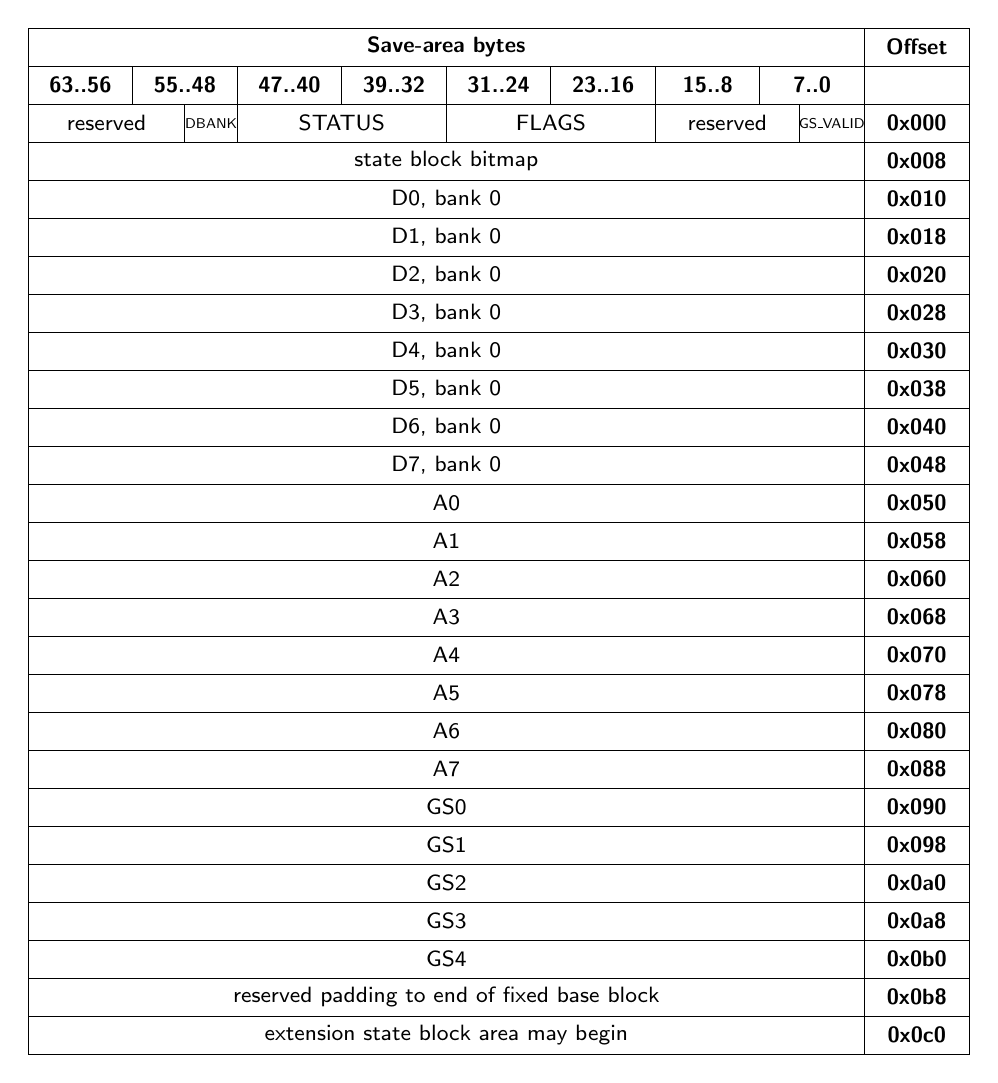
\begin{tikzpicture}[x=0.01368\linewidth,y=0.19in,every node/.style={font=\footnotesize,inner sep=1pt,align=center}]
\draw[line width=0.35pt] (0,0) rectangle (64,-1);
\node[font=\bfseries\footnotesize] at (32,-0.5) {Save-area bytes};
\draw[line width=0.35pt] (64,0) rectangle (72,-1);
\node[font=\bfseries\footnotesize] at (68,-0.5) {Offset};
\draw[line width=0.35pt] (0,-1) rectangle (8,-2);
\node[font=\bfseries\footnotesize] at (4,-1.5) {63..56};
\draw[line width=0.35pt] (8,-1) rectangle (16,-2);
\node[font=\bfseries\footnotesize] at (12,-1.5) {55..48};
\draw[line width=0.35pt] (16,-1) rectangle (24,-2);
\node[font=\bfseries\footnotesize] at (20,-1.5) {47..40};
\draw[line width=0.35pt] (24,-1) rectangle (32,-2);
\node[font=\bfseries\footnotesize] at (28,-1.5) {39..32};
\draw[line width=0.35pt] (32,-1) rectangle (40,-2);
\node[font=\bfseries\footnotesize] at (36,-1.5) {31..24};
\draw[line width=0.35pt] (40,-1) rectangle (48,-2);
\node[font=\bfseries\footnotesize] at (44,-1.5) {23..16};
\draw[line width=0.35pt] (48,-1) rectangle (56,-2);
\node[font=\bfseries\footnotesize] at (52,-1.5) {15..8};
\draw[line width=0.35pt] (56,-1) rectangle (64,-2);
\node[font=\bfseries\footnotesize] at (60,-1.5) {7..0};
\draw[line width=0.35pt] (64,-1) rectangle (72,-2);
\draw[line width=0.35pt] (0,-2) rectangle (12,-3);
\node at (6.00,-2.50) {reserved};
\draw[line width=0.35pt] (12,-2) rectangle (16,-3);
\node[scale=0.64] at (14.00,-2.50) {DBANK};
\draw[line width=0.35pt] (16,-2) rectangle (32,-3);
\node at (24.00,-2.50) {STATUS};
\draw[line width=0.35pt] (32,-2) rectangle (48,-3);
\node at (40.00,-2.50) {FLAGS};
\draw[line width=0.35pt] (48,-2) rectangle (59,-3);
\node at (53.50,-2.50) {reserved};
\draw[line width=0.35pt] (59,-2) rectangle (64,-3);
\node[scale=0.64] at (61.50,-2.50) {GS\_VALID};
\draw[line width=0.35pt] (64,-2) rectangle (72,-3);
\node[font=\bfseries\footnotesize] at (68,-2.50) {0x000};
\draw[line width=0.35pt] (0,-3) rectangle (64,-4);
\node at (32.00,-3.50) {state block bitmap};
\draw[line width=0.35pt] (64,-3) rectangle (72,-4);
\node[font=\bfseries\footnotesize] at (68,-3.50) {0x008};
\draw[line width=0.35pt] (0,-4) rectangle (64,-5);
\node at (32.00,-4.50) {D0, bank 0};
\draw[line width=0.35pt] (64,-4) rectangle (72,-5);
\node[font=\bfseries\footnotesize] at (68,-4.50) {0x010};
\draw[line width=0.35pt] (0,-5) rectangle (64,-6);
\node at (32.00,-5.50) {D1, bank 0};
\draw[line width=0.35pt] (64,-5) rectangle (72,-6);
\node[font=\bfseries\footnotesize] at (68,-5.50) {0x018};
\draw[line width=0.35pt] (0,-6) rectangle (64,-7);
\node at (32.00,-6.50) {D2, bank 0};
\draw[line width=0.35pt] (64,-6) rectangle (72,-7);
\node[font=\bfseries\footnotesize] at (68,-6.50) {0x020};
\draw[line width=0.35pt] (0,-7) rectangle (64,-8);
\node at (32.00,-7.50) {D3, bank 0};
\draw[line width=0.35pt] (64,-7) rectangle (72,-8);
\node[font=\bfseries\footnotesize] at (68,-7.50) {0x028};
\draw[line width=0.35pt] (0,-8) rectangle (64,-9);
\node at (32.00,-8.50) {D4, bank 0};
\draw[line width=0.35pt] (64,-8) rectangle (72,-9);
\node[font=\bfseries\footnotesize] at (68,-8.50) {0x030};
\draw[line width=0.35pt] (0,-9) rectangle (64,-10);
\node at (32.00,-9.50) {D5, bank 0};
\draw[line width=0.35pt] (64,-9) rectangle (72,-10);
\node[font=\bfseries\footnotesize] at (68,-9.50) {0x038};
\draw[line width=0.35pt] (0,-10) rectangle (64,-11);
\node at (32.00,-10.50) {D6, bank 0};
\draw[line width=0.35pt] (64,-10) rectangle (72,-11);
\node[font=\bfseries\footnotesize] at (68,-10.50) {0x040};
\draw[line width=0.35pt] (0,-11) rectangle (64,-12);
\node at (32.00,-11.50) {D7, bank 0};
\draw[line width=0.35pt] (64,-11) rectangle (72,-12);
\node[font=\bfseries\footnotesize] at (68,-11.50) {0x048};
\draw[line width=0.35pt] (0,-12) rectangle (64,-13);
\node at (32.00,-12.50) {A0};
\draw[line width=0.35pt] (64,-12) rectangle (72,-13);
\node[font=\bfseries\footnotesize] at (68,-12.50) {0x050};
\draw[line width=0.35pt] (0,-13) rectangle (64,-14);
\node at (32.00,-13.50) {A1};
\draw[line width=0.35pt] (64,-13) rectangle (72,-14);
\node[font=\bfseries\footnotesize] at (68,-13.50) {0x058};
\draw[line width=0.35pt] (0,-14) rectangle (64,-15);
\node at (32.00,-14.50) {A2};
\draw[line width=0.35pt] (64,-14) rectangle (72,-15);
\node[font=\bfseries\footnotesize] at (68,-14.50) {0x060};
\draw[line width=0.35pt] (0,-15) rectangle (64,-16);
\node at (32.00,-15.50) {A3};
\draw[line width=0.35pt] (64,-15) rectangle (72,-16);
\node[font=\bfseries\footnotesize] at (68,-15.50) {0x068};
\draw[line width=0.35pt] (0,-16) rectangle (64,-17);
\node at (32.00,-16.50) {A4};
\draw[line width=0.35pt] (64,-16) rectangle (72,-17);
\node[font=\bfseries\footnotesize] at (68,-16.50) {0x070};
\draw[line width=0.35pt] (0,-17) rectangle (64,-18);
\node at (32.00,-17.50) {A5};
\draw[line width=0.35pt] (64,-17) rectangle (72,-18);
\node[font=\bfseries\footnotesize] at (68,-17.50) {0x078};
\draw[line width=0.35pt] (0,-18) rectangle (64,-19);
\node at (32.00,-18.50) {A6};
\draw[line width=0.35pt] (64,-18) rectangle (72,-19);
\node[font=\bfseries\footnotesize] at (68,-18.50) {0x080};
\draw[line width=0.35pt] (0,-19) rectangle (64,-20);
\node at (32.00,-19.50) {A7};
\draw[line width=0.35pt] (64,-19) rectangle (72,-20);
\node[font=\bfseries\footnotesize] at (68,-19.50) {0x088};
\draw[line width=0.35pt] (0,-20) rectangle (64,-21);
\node at (32.00,-20.50) {GS0};
\draw[line width=0.35pt] (64,-20) rectangle (72,-21);
\node[font=\bfseries\footnotesize] at (68,-20.50) {0x090};
\draw[line width=0.35pt] (0,-21) rectangle (64,-22);
\node at (32.00,-21.50) {GS1};
\draw[line width=0.35pt] (64,-21) rectangle (72,-22);
\node[font=\bfseries\footnotesize] at (68,-21.50) {0x098};
\draw[line width=0.35pt] (0,-22) rectangle (64,-23);
\node at (32.00,-22.50) {GS2};
\draw[line width=0.35pt] (64,-22) rectangle (72,-23);
\node[font=\bfseries\footnotesize] at (68,-22.50) {0x0a0};
\draw[line width=0.35pt] (0,-23) rectangle (64,-24);
\node at (32.00,-23.50) {GS3};
\draw[line width=0.35pt] (64,-23) rectangle (72,-24);
\node[font=\bfseries\footnotesize] at (68,-23.50) {0x0a8};
\draw[line width=0.35pt] (0,-24) rectangle (64,-25);
\node at (32.00,-24.50) {GS4};
\draw[line width=0.35pt] (64,-24) rectangle (72,-25);
\node[font=\bfseries\footnotesize] at (68,-24.50) {0x0b0};
\draw[line width=0.35pt] (0,-25) rectangle (64,-26);
\node at (32.00,-25.50) {reserved padding to end of fixed base block};
\draw[line width=0.35pt] (64,-25) rectangle (72,-26);
\node[font=\bfseries\footnotesize] at (68,-25.50) {0x0b8};
\draw[line width=0.35pt] (0,-26) rectangle (64,-27);
\node at (32.00,-26.50) {extension state block area may begin};
\draw[line width=0.35pt] (64,-26) rectangle (72,-27);
\node[font=\bfseries\footnotesize] at (68,-26.50) {0x0c0};
\end{tikzpicture}\par\smallskip
\Needspace{2.40in}
\noindent\textbf{Base Header Fields:}\par\smallskip\noindent
\begingroup\footnotesize\renewcommand{\arraystretch}{1.08}
\begin{tabularx}{0.985\linewidth}{|p{0.56in}|p{0.62in}|p{1.35in}|X|}
\hline
\textbf{Offset} & \textbf{Bits} & \textbf{Field} & \textbf{Meaning}\\
\hline
0x000 & 0..4 & GS\_VALID & bit n validates GSn at 0x090 + 8*n; RESTORE updates only GS slots whose bits are set\\
\hline
0x000 & 5..15 & reserved & SAVE writes zero and RESTORE ignores\\
\hline
0x000 & 16..31 & FLAGS & always-saved integer condition-code FLAGS image\\
\hline
0x000 & 32..47 & STATUS & always-saved STATUS image; user-mode RESTORE ignores this field, supervisor RESTORE applies STATUS write rules\\
\hline
0x000 & 48..51 & DBANK & current data-register bank selector; RESTORE applies the SELDB validity rules and updates the selector after bank payloads\\
\hline
0x000 & 52..63 & reserved & SAVE writes zero and RESTORE ignores\\
\hline
0x008 & i & component descriptor 2+i present & i=0..SAVE\_COMPONENT\_COUNT-1 and SAVE\_COMPONENT\_COUNT must be no larger than 64\\
\hline
0x008 & all other bits & reserved & SAVE writes zero and RESTORE ignores\\
\hline
\end{tabularx}\endgroup\par\smallskip
\noindent SAVE always writes the base header fields, state block bitmap, bank-0 D registers, A registers, FLAGS, STATUS, and DBANK selector. SAVE may clear GS validity bits for architecturally clean GS slots and may clear state-block bitmap bits for architecturally clean extension blocks. RESTORE always restores bank-0 D registers, A registers, FLAGS, and DBANK from the fixed base block. RESTORE updates only GS slots whose GS validity bit is set. User-mode RESTORE ignores the STATUS field and does not validate STATUS reserved bits; supervisor RESTORE restores STATUS under the normal STATUS write rules. RESTORE processes extension blocks whose state-block bitmap bit is set and ignores blocks whose bit is clear.\par
\noindent Extension component offsets begin no earlier than SAVE\_HEADER\_SIZE, 0x0c0 for the base profile, and are reported by CPUID. The save-area base address is 4 KiB aligned. Every component offset and component storage size is a multiple of 64 bytes so state blocks are cache-line aligned.\par
\noindent CPUID SAVE\_AREA\_LAYOUT component descriptors are indexed from 2 upward. That descriptor index order is the architectural extension-component order and is the bit order used by the fixed state block bitmap at offset 0x008. COMPONENT\_OFFSET values are numeric byte offsets and must be strictly increasing in descriptor order. Base-defined component formats appear first; extension-owned component formats are appended by descriptor order from their owning extension specs. The SAVE area has no architectural total-size upper bound beyond the CPUID-reported SAVE\_AREA\_SIZE value for the selected implementation/profile, but SAVE\_COMPONENT\_COUNT is limited to 64 by the fixed state block bitmap.\par
\par\smallskip\noindent\textbf{Extension Component Formats:}\par
\par\smallskip\Needspace{2.4in}
\noindent\textbf{Extension Component: Additional Data-Register Banks}\par\smallskip
\begingroup\footnotesize
\begin{tabularx}{0.985\linewidth}{@{}p{1.35in}X@{}}
\textbf{Component ID} & 0x0001\\
\textbf{Component Name} & \texttt{DATA\_REGISTER\_BANKS}\\
\textbf{Component Size} & 0x40 * DBANK\_COUNT\\
\end{tabularx}\endgroup\par\smallskip
\noindent This component stores data-register banks other than bank 0. Bank 0 is part of the fixed base block. The first 64 bytes are the component header. Each following 0x40-byte bank record stores D0-D7 for the matching bank number and begins on a 64-byte boundary.\par\smallskip
\noindent The component header fields contain a bank-level validity bitmap. If a bank bit is clear, RESTORE leaves that nonzero D-register bank unchanged.\par\smallskip
\Needspace{1.48in}
\noindent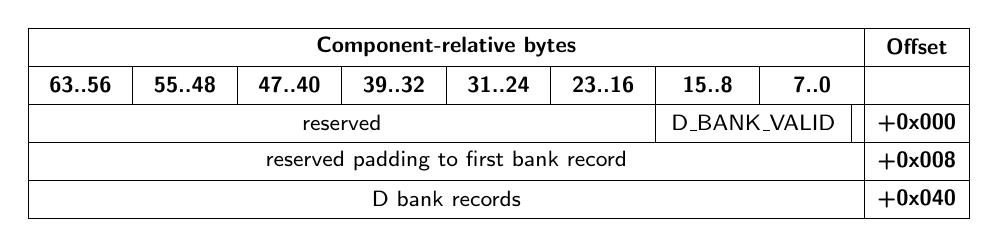
\begin{tikzpicture}[x=0.01368\linewidth,y=0.19in,every node/.style={font=\footnotesize,inner sep=1pt,align=center}]
\draw[line width=0.35pt] (0,0) rectangle (64,-1);
\node[font=\bfseries\footnotesize] at (32,-0.5) {Component-relative bytes};
\draw[line width=0.35pt] (64,0) rectangle (72,-1);
\node[font=\bfseries\footnotesize] at (68,-0.5) {Offset};
\draw[line width=0.35pt] (0,-1) rectangle (8,-2);
\node[font=\bfseries\footnotesize] at (4,-1.5) {63..56};
\draw[line width=0.35pt] (8,-1) rectangle (16,-2);
\node[font=\bfseries\footnotesize] at (12,-1.5) {55..48};
\draw[line width=0.35pt] (16,-1) rectangle (24,-2);
\node[font=\bfseries\footnotesize] at (20,-1.5) {47..40};
\draw[line width=0.35pt] (24,-1) rectangle (32,-2);
\node[font=\bfseries\footnotesize] at (28,-1.5) {39..32};
\draw[line width=0.35pt] (32,-1) rectangle (40,-2);
\node[font=\bfseries\footnotesize] at (36,-1.5) {31..24};
\draw[line width=0.35pt] (40,-1) rectangle (48,-2);
\node[font=\bfseries\footnotesize] at (44,-1.5) {23..16};
\draw[line width=0.35pt] (48,-1) rectangle (56,-2);
\node[font=\bfseries\footnotesize] at (52,-1.5) {15..8};
\draw[line width=0.35pt] (56,-1) rectangle (64,-2);
\node[font=\bfseries\footnotesize] at (60,-1.5) {7..0};
\draw[line width=0.35pt] (64,-1) rectangle (72,-2);
\draw[line width=0.35pt] (0,-2) rectangle (48,-3);
\node at (24.00,-2.50) {reserved};
\draw[line width=0.35pt] (48,-2) rectangle (63,-3);
\node at (55.50,-2.50) {D\_BANK\_VALID};
\draw[line width=0.35pt] (63,-2) rectangle (64,-3);
\draw[line width=0.35pt] (64,-2) rectangle (72,-3);
\node[font=\bfseries\footnotesize] at (68,-2.50) {+0x000};
\draw[line width=0.35pt] (0,-3) rectangle (64,-4);
\node at (32.00,-3.50) {reserved padding to first bank record};
\draw[line width=0.35pt] (64,-3) rectangle (72,-4);
\node[font=\bfseries\footnotesize] at (68,-3.50) {+0x008};
\draw[line width=0.35pt] (0,-4) rectangle (64,-5);
\node at (32.00,-4.50) {D bank records};
\draw[line width=0.35pt] (64,-4) rectangle (72,-5);
\node[font=\bfseries\footnotesize] at (68,-4.50) {+0x040};
\end{tikzpicture}\par\smallskip
\Needspace{1.27in}
\noindent\textbf{Component Header Fields:}\par\smallskip\noindent
\begingroup\footnotesize\renewcommand{\arraystretch}{1.08}
\begin{tabularx}{0.985\linewidth}{|p{0.56in}|p{0.62in}|p{1.35in}|X|}
\hline
\textbf{Offset} & \textbf{Bits} & \textbf{Field} & \textbf{Meaning}\\
\hline
+0x000 & 0 & reserved & bank 0 lives in the fixed base block\\
\hline
+0x000 & 1..15 & D\_BANK\_VALID & bit b validates D bank b at +0x040*b for b=1..DBANK\_COUNT-1\\
\hline
+0x000 & 16..63 & reserved & bits for unimplemented banks and future state are reserved\\
\hline
\end{tabularx}\endgroup\par\smallskip
\par\smallskip\Needspace{2.4in}
\noindent\textbf{Extension Component: Floating-Point State}\par\smallskip
\begingroup\footnotesize
\begin{tabularx}{0.985\linewidth}{@{}p{1.35in}X@{}}
\textbf{Component ID} & 0x0002\\
\textbf{Component Name} & \texttt{FLOATING\_POINT}\\
\textbf{Extension Requirement} & \texttt{floating\_point}\\
\textbf{Component Size} & 0x00c0\\
\end{tabularx}\endgroup\par\smallskip
\noindent This component stores the floating-point accrued exception flags, the floating-point status/control-mode word, and the architectural floating-point register file. The first 64-bit word packs the F-register validity bitmap together with FFLAGS and FSTATUS. The F register file starts at +0x008 and the component storage size is rounded up to a 64-byte boundary.\par\smallskip
\noindent The component header contains the F-register validity bitmap. FFLAGS and FSTATUS are present whenever the floating-point state block is present.\par\smallskip
\Needspace{4.48in}
\noindent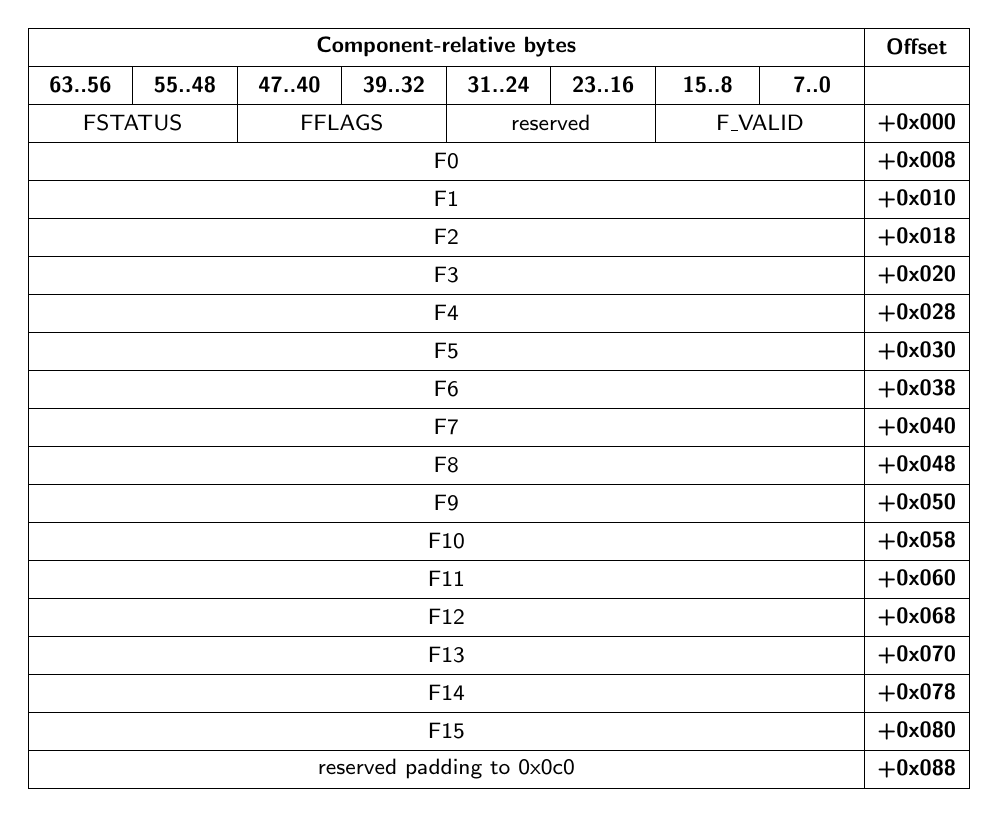
\begin{tikzpicture}[x=0.01368\linewidth,y=0.19in,every node/.style={font=\footnotesize,inner sep=1pt,align=center}]
\draw[line width=0.35pt] (0,0) rectangle (64,-1);
\node[font=\bfseries\footnotesize] at (32,-0.5) {Component-relative bytes};
\draw[line width=0.35pt] (64,0) rectangle (72,-1);
\node[font=\bfseries\footnotesize] at (68,-0.5) {Offset};
\draw[line width=0.35pt] (0,-1) rectangle (8,-2);
\node[font=\bfseries\footnotesize] at (4,-1.5) {63..56};
\draw[line width=0.35pt] (8,-1) rectangle (16,-2);
\node[font=\bfseries\footnotesize] at (12,-1.5) {55..48};
\draw[line width=0.35pt] (16,-1) rectangle (24,-2);
\node[font=\bfseries\footnotesize] at (20,-1.5) {47..40};
\draw[line width=0.35pt] (24,-1) rectangle (32,-2);
\node[font=\bfseries\footnotesize] at (28,-1.5) {39..32};
\draw[line width=0.35pt] (32,-1) rectangle (40,-2);
\node[font=\bfseries\footnotesize] at (36,-1.5) {31..24};
\draw[line width=0.35pt] (40,-1) rectangle (48,-2);
\node[font=\bfseries\footnotesize] at (44,-1.5) {23..16};
\draw[line width=0.35pt] (48,-1) rectangle (56,-2);
\node[font=\bfseries\footnotesize] at (52,-1.5) {15..8};
\draw[line width=0.35pt] (56,-1) rectangle (64,-2);
\node[font=\bfseries\footnotesize] at (60,-1.5) {7..0};
\draw[line width=0.35pt] (64,-1) rectangle (72,-2);
\draw[line width=0.35pt] (0,-2) rectangle (16,-3);
\node at (8.00,-2.50) {FSTATUS};
\draw[line width=0.35pt] (16,-2) rectangle (32,-3);
\node at (24.00,-2.50) {FFLAGS};
\draw[line width=0.35pt] (32,-2) rectangle (48,-3);
\node at (40.00,-2.50) {reserved};
\draw[line width=0.35pt] (48,-2) rectangle (64,-3);
\node at (56.00,-2.50) {F\_VALID};
\draw[line width=0.35pt] (64,-2) rectangle (72,-3);
\node[font=\bfseries\footnotesize] at (68,-2.50) {+0x000};
\draw[line width=0.35pt] (0,-3) rectangle (64,-4);
\node at (32.00,-3.50) {F0};
\draw[line width=0.35pt] (64,-3) rectangle (72,-4);
\node[font=\bfseries\footnotesize] at (68,-3.50) {+0x008};
\draw[line width=0.35pt] (0,-4) rectangle (64,-5);
\node at (32.00,-4.50) {F1};
\draw[line width=0.35pt] (64,-4) rectangle (72,-5);
\node[font=\bfseries\footnotesize] at (68,-4.50) {+0x010};
\draw[line width=0.35pt] (0,-5) rectangle (64,-6);
\node at (32.00,-5.50) {F2};
\draw[line width=0.35pt] (64,-5) rectangle (72,-6);
\node[font=\bfseries\footnotesize] at (68,-5.50) {+0x018};
\draw[line width=0.35pt] (0,-6) rectangle (64,-7);
\node at (32.00,-6.50) {F3};
\draw[line width=0.35pt] (64,-6) rectangle (72,-7);
\node[font=\bfseries\footnotesize] at (68,-6.50) {+0x020};
\draw[line width=0.35pt] (0,-7) rectangle (64,-8);
\node at (32.00,-7.50) {F4};
\draw[line width=0.35pt] (64,-7) rectangle (72,-8);
\node[font=\bfseries\footnotesize] at (68,-7.50) {+0x028};
\draw[line width=0.35pt] (0,-8) rectangle (64,-9);
\node at (32.00,-8.50) {F5};
\draw[line width=0.35pt] (64,-8) rectangle (72,-9);
\node[font=\bfseries\footnotesize] at (68,-8.50) {+0x030};
\draw[line width=0.35pt] (0,-9) rectangle (64,-10);
\node at (32.00,-9.50) {F6};
\draw[line width=0.35pt] (64,-9) rectangle (72,-10);
\node[font=\bfseries\footnotesize] at (68,-9.50) {+0x038};
\draw[line width=0.35pt] (0,-10) rectangle (64,-11);
\node at (32.00,-10.50) {F7};
\draw[line width=0.35pt] (64,-10) rectangle (72,-11);
\node[font=\bfseries\footnotesize] at (68,-10.50) {+0x040};
\draw[line width=0.35pt] (0,-11) rectangle (64,-12);
\node at (32.00,-11.50) {F8};
\draw[line width=0.35pt] (64,-11) rectangle (72,-12);
\node[font=\bfseries\footnotesize] at (68,-11.50) {+0x048};
\draw[line width=0.35pt] (0,-12) rectangle (64,-13);
\node at (32.00,-12.50) {F9};
\draw[line width=0.35pt] (64,-12) rectangle (72,-13);
\node[font=\bfseries\footnotesize] at (68,-12.50) {+0x050};
\draw[line width=0.35pt] (0,-13) rectangle (64,-14);
\node at (32.00,-13.50) {F10};
\draw[line width=0.35pt] (64,-13) rectangle (72,-14);
\node[font=\bfseries\footnotesize] at (68,-13.50) {+0x058};
\draw[line width=0.35pt] (0,-14) rectangle (64,-15);
\node at (32.00,-14.50) {F11};
\draw[line width=0.35pt] (64,-14) rectangle (72,-15);
\node[font=\bfseries\footnotesize] at (68,-14.50) {+0x060};
\draw[line width=0.35pt] (0,-15) rectangle (64,-16);
\node at (32.00,-15.50) {F12};
\draw[line width=0.35pt] (64,-15) rectangle (72,-16);
\node[font=\bfseries\footnotesize] at (68,-15.50) {+0x068};
\draw[line width=0.35pt] (0,-16) rectangle (64,-17);
\node at (32.00,-16.50) {F13};
\draw[line width=0.35pt] (64,-16) rectangle (72,-17);
\node[font=\bfseries\footnotesize] at (68,-16.50) {+0x070};
\draw[line width=0.35pt] (0,-17) rectangle (64,-18);
\node at (32.00,-17.50) {F14};
\draw[line width=0.35pt] (64,-17) rectangle (72,-18);
\node[font=\bfseries\footnotesize] at (68,-17.50) {+0x078};
\draw[line width=0.35pt] (0,-18) rectangle (64,-19);
\node at (32.00,-18.50) {F15};
\draw[line width=0.35pt] (64,-18) rectangle (72,-19);
\node[font=\bfseries\footnotesize] at (68,-18.50) {+0x080};
\draw[line width=0.35pt] (0,-19) rectangle (64,-20);
\node at (32.00,-19.50) {reserved padding to 0x0c0};
\draw[line width=0.35pt] (64,-19) rectangle (72,-20);
\node[font=\bfseries\footnotesize] at (68,-19.50) {+0x088};
\end{tikzpicture}\par\smallskip
\Needspace{1.51in}
\noindent\textbf{Component Header Fields:}\par\smallskip\noindent
\begingroup\footnotesize\renewcommand{\arraystretch}{1.08}
\begin{tabularx}{0.985\linewidth}{|p{0.56in}|p{0.62in}|p{1.35in}|X|}
\hline
\textbf{Offset} & \textbf{Bits} & \textbf{Field} & \textbf{Meaning}\\
\hline
+0x000 & 0..15 & F\_VALID & bit n validates Fn at +0x008 + 8*n\\
\hline
+0x000 & 16..31 & reserved & SAVE writes zero and RESTORE ignores\\
\hline
+0x000 & 32..47 & FFLAGS & floating-point accrued exception flags, always present when this state block is present\\
\hline
+0x000 & 48..63 & FSTATUS & floating-point control and status-mode register, always present when this state block is present\\
\hline
\end{tabularx}\endgroup\par\smallskip
\smallskip
\end{document}
